\section{Model}
In this section the model of \projectname{} will be presented and explained.
First the objects that needs to be represented by the model are identified, and then their relationships will be described.

\subsection{Objects}
\label{subsec:objects}
\fixme{This might fit better in the analysis}
The core aspects that must be represented is users and drones.
A users' access to the system will need to be restricted.
This restriction will be represented through privileges that grant a user access to system functionalities.
Granting privileges directly to a user is not the ideal case in most situations.
The system will contain global privileges all users need access to.
Assigning global privileges to each user individually is not an ideal solution.
Therefore this will be handled via roles.
A role will in \projectname{} be a set of privileges and assignable to multiple users.

A drone is controlled by sending a set of ordered instructions\fixme{ref to section when it is written} to the drone.
A log of flights made by the drone will need to be kept, to be able to recreate previous flights, and examine a flight that might have caused the drone to crash.
This log will be referenced in the system as a flight plan.
A flight plan will consist of a set of actions taken by the drone, each referencing a specific instruction send to the drone.

A structured list of the object can be seen in Figure~\ref{tab:model_objects}.

\begin{figure}[H]
\begin{center}
\begin{tabular}{ |c| }
  \hline              
	\textbf{Object}\\ \hline
	User \\ \hline
	Role \\ \hline
	Privilege \\ \hline
	Drone \\ \hline
	Flight plan \\ \hline
	Action \\ \hline
	Instruction\\ \hline  
\end{tabular}
\caption{Use Cases}
\label{tab:model_objects}
\end{center}
\end{figure}

\subsection{Model Diagram}
A diagram of the model can be seen in Figure~\ref{}\fixme{inds�t figur}.
It should be noted all tables are named according to the standard in Ruby\fixme{Source til Ruby naming convention}
The upper part of figure describes the relationship between users, roles, and privileges.

\subsubsection{User Privilege Relationship}
As mentioned in Section~\ref{subsec:objects} a role in \projectname{} is a set of privileges.
A role is linked to a set of privileges through the relationship table \verb+Privilege_roles+.
In Rails this relationship is referred to as a many to many association, as a user can be associated with many roles and a role can be associated with many users.
\verb+Privilege_roles+ links the ids of roles to the ids of privileges.
Users and roles a linked in the same manner as roles and privileges.
In the table \verb+Role_Users+ the ids of users to the ids of roles are linked\fixme{M�ske sample model der viser princippet hvis det er for upr�cist}.
\begin{figure}[htb]
    \centering
    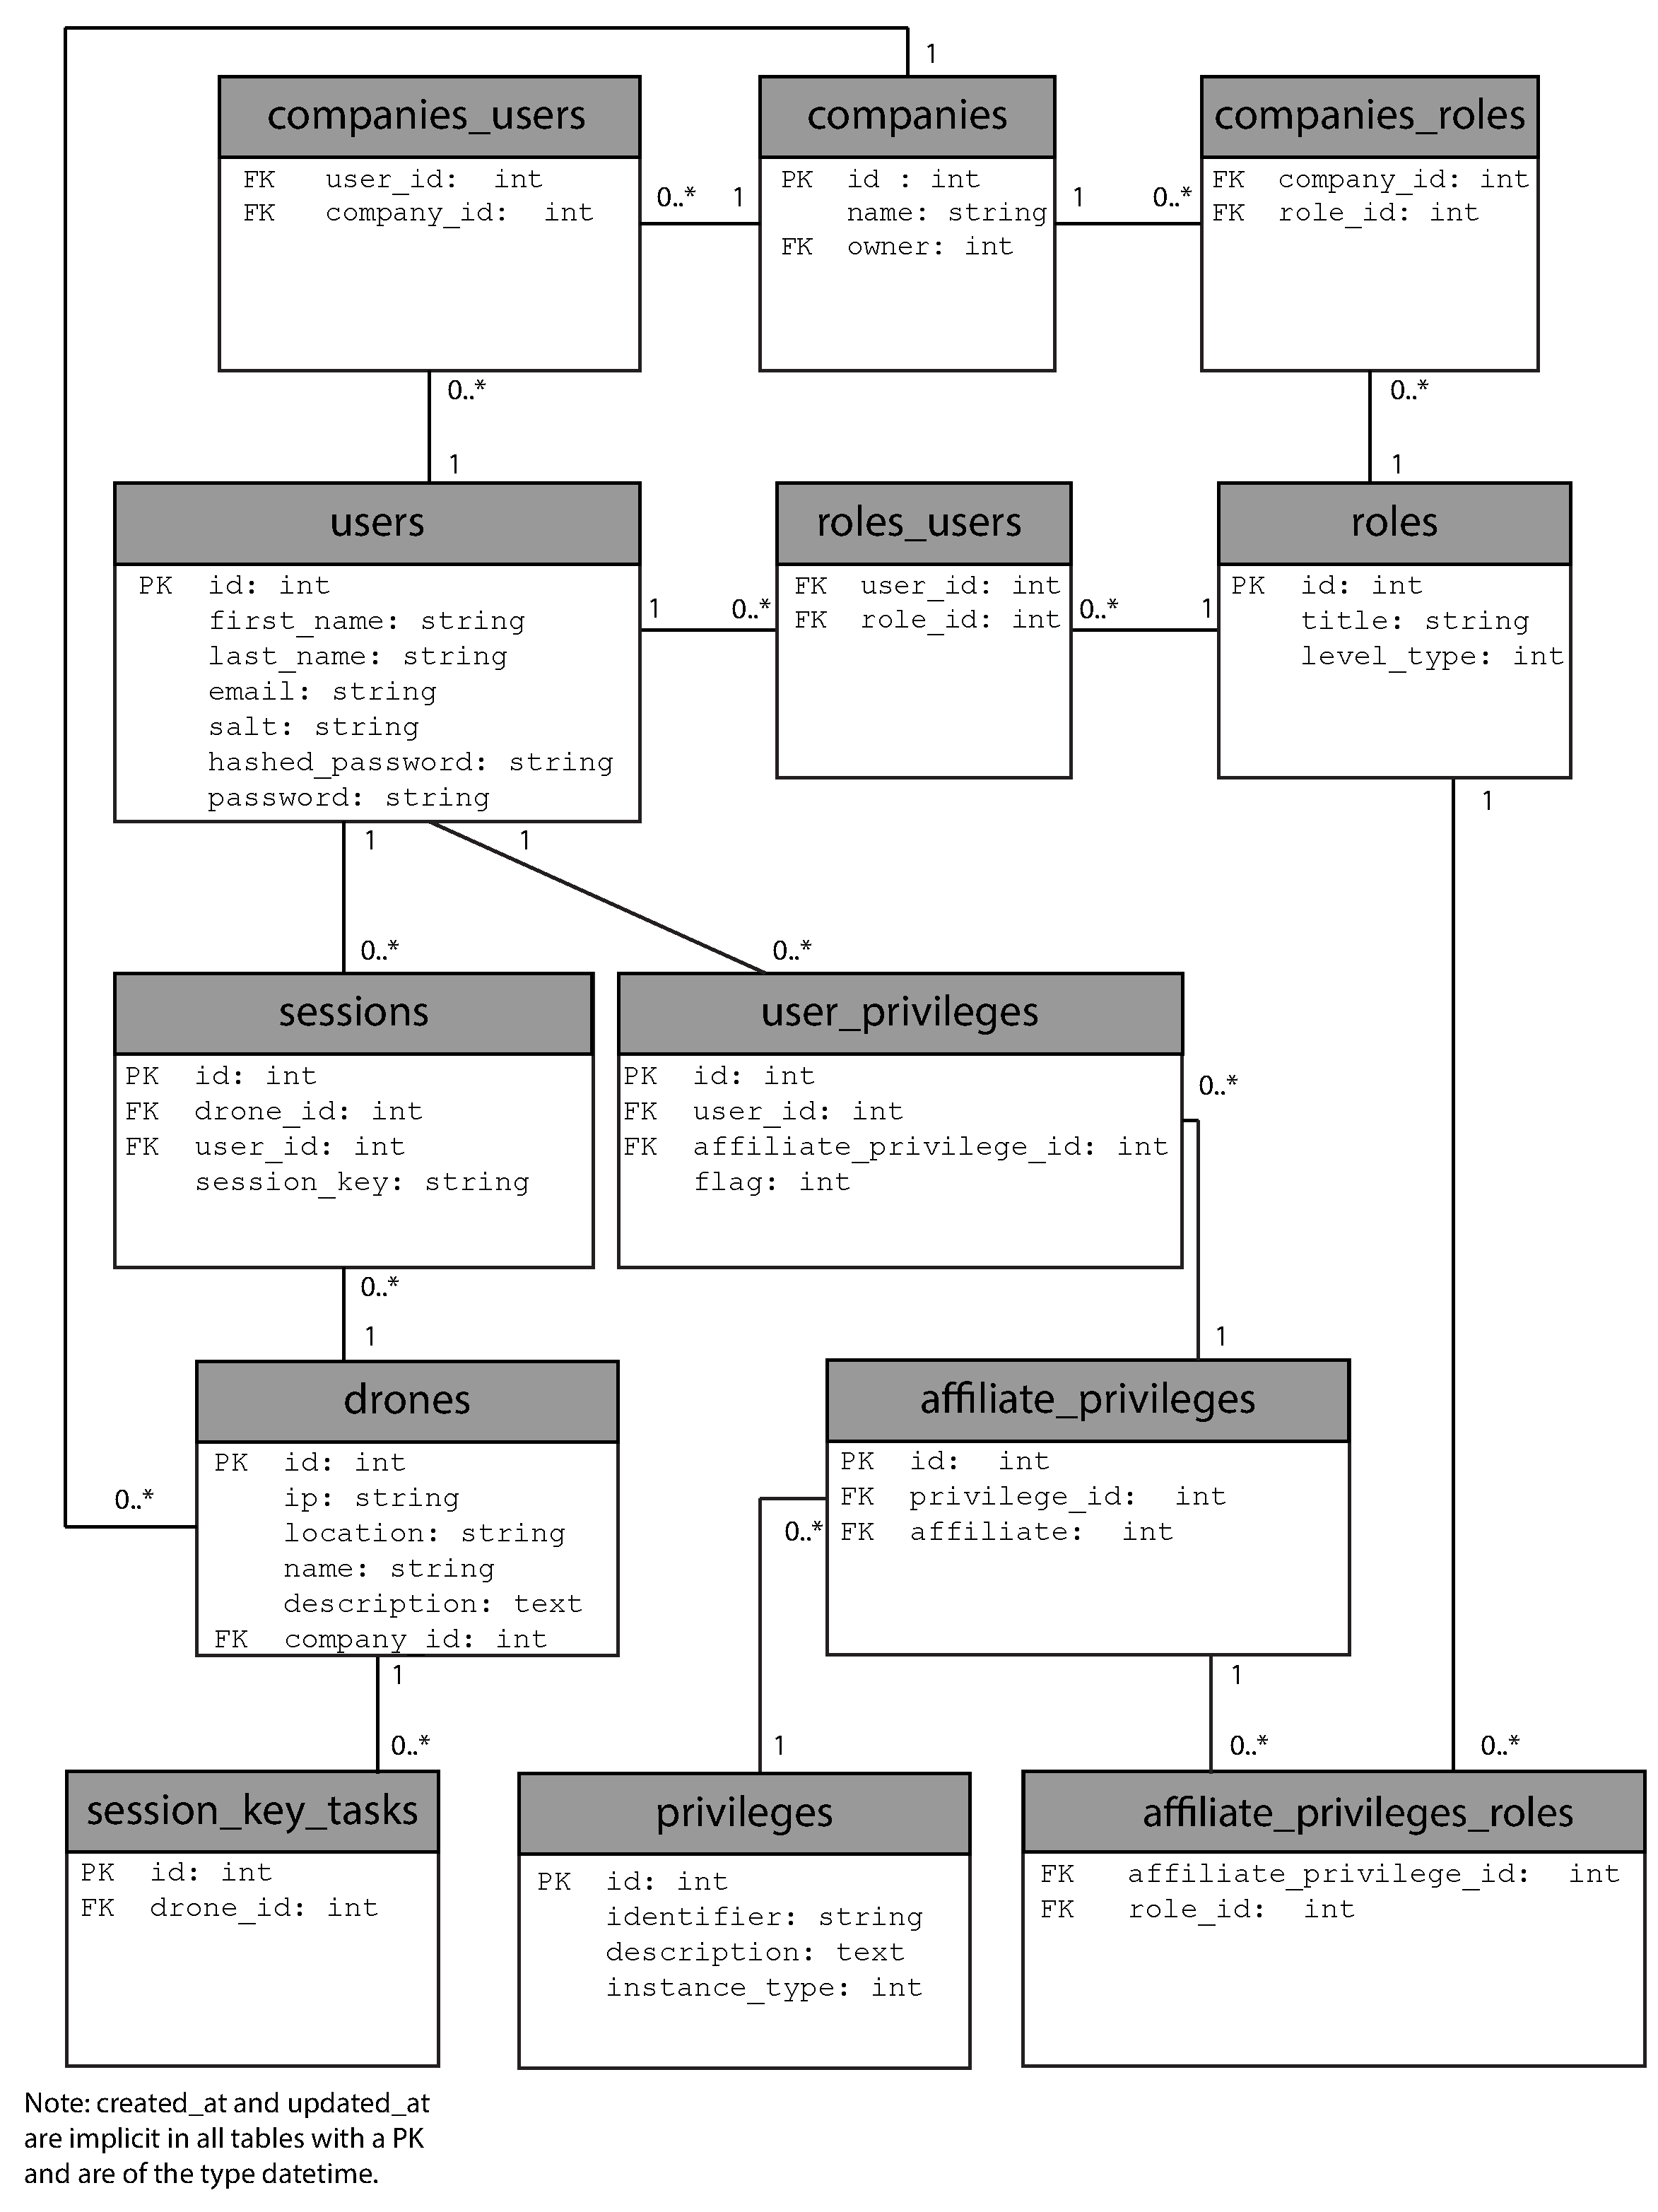
\includegraphics[width=\textwidth]{gfx/UML_model.pdf}
    \caption{UML Class Diagram of \projectname{}}
    \label{fig:UML_class_diagram}
\end{figure}

However linking privileges to users only through roles creates cases were maintaining privileges can become troublesome.
As an example a user \verb+u+ might need to have his access to a specific privilege \verb+p+ in a role \verb+r+, he is a member of, revoked.
A possible solution is to remove the user from \verb+r+ and add him a to new role \verb+r1+ that contains all privileges in \verb+r+ except \verb+p+.
The problem with this solution arises if a new privilege \verb+p1+ is to be added to \verb+r+.
The user \verb+u+ is implicitly a member of \verb+r+, but has the role \verb+r1+ to exclude him from the privilege \verb+p+.
To grant \verb+u+ \verb+p1+, \verb+p1+ must be added to \verb+r1+ as well as \verb+r+.
Granting privileges only through roles can therefore quickly result in a lot of unstructured data that needs to be maintained.

To handle this users are linked directly to privileges through the relationship table \verb+User_Privileges+.
This table differs from the other relationship tables as it does not just link to id foreign keys.
In Rails this is referred to as a rich many to many associated.
In a rich many to many associated additional fields are added to the relationship table.
In \verb+User_Privileges+ users and privileges are linked through ids, with an extra field containing a flag.
This flag defines if the privilege the user is linked to is whitelisted or blacklisted through the relation.
The design makes management of privileges more flexible.
Groups of privileges can be assigned through roles, and should a case arise where a users privileges needs to be managed individually this is possible through the \verb+User_Privileges+ relation.

\subsection{Drone Flight Plan Relationship}
The flight logging system consists directly of the classes \verb+Drones+, \verb+Flight_plan+, and \verb+Actions+.
Drones are linked to flight plans through a foreign key.
A flight plan is connected to a set of actions through a one to many relation.
The actions must be numbered representing the order in which the actions were send to the drone.
This numbering will be managed in the \verb+Flight_Action_Relationship+\fixme{Opdater dette n�r den gives et nyt navn} with the field \verb+rank+.
An action will be linked to an instruction.
Instruction represent the set of AT commands which can be send to the drone to control.\fixme{Ref til AT command sektion n�r den skrives}

Through this model the log for a flight with a given drone can be extracted by locating all action associated with the flight plan through the \verb+Flight_Action_Relationship+.



%\subsection{Privileges}
%A user is granted privileges through a whitelist.
%Every privilege not found in a users whitelist is implicitly blacklisted.
%As described in Section~\ref{subsec:objects} a user can be granted privileges through roles.
%There are however a set of cases where handling privileges only through roles is not ideal.
%As an example a user \verb+u+ might need to have his access to a specific privilege \verb+p+ in a role \verb+r+, he is a member of, revoked.
%A possible solution is to remove the user from \verb+r+ and add him a to new role \verb+r1+ that contains all privileges in \verb+r+ except \verb+p+.
%The problem with this solution arises if a new privilege \verb+p1+ is to be added to \verb+r+.
%The user \verb+u+ is natively a member of \verb+r+, but has the role \verb+r1+ to exclude him from the privilege \verb+p+.
%To grant \verb+u+ \verb+p1+, \verb+p1+ must be added to \verb+r1+ as well as \verb+r+.
%Granting privileges only through roles can therefore quickly result in a lot of unstructured data that needs to be maintained.
%To solve privileges need to be manageable on the user level.


%As an example a user might need a specific privilege that allows him to fly a specific drone.
%Adding the user to a group \verb+p+ with that privilege would not work as he would then additionally receive every other privilege in \verb+p+.
%The problem can be solved by giving each user a personal role containing all their uniquely assigned privileges.